\documentclass[tikz,border=10pt]{standalone}
\begin{document}
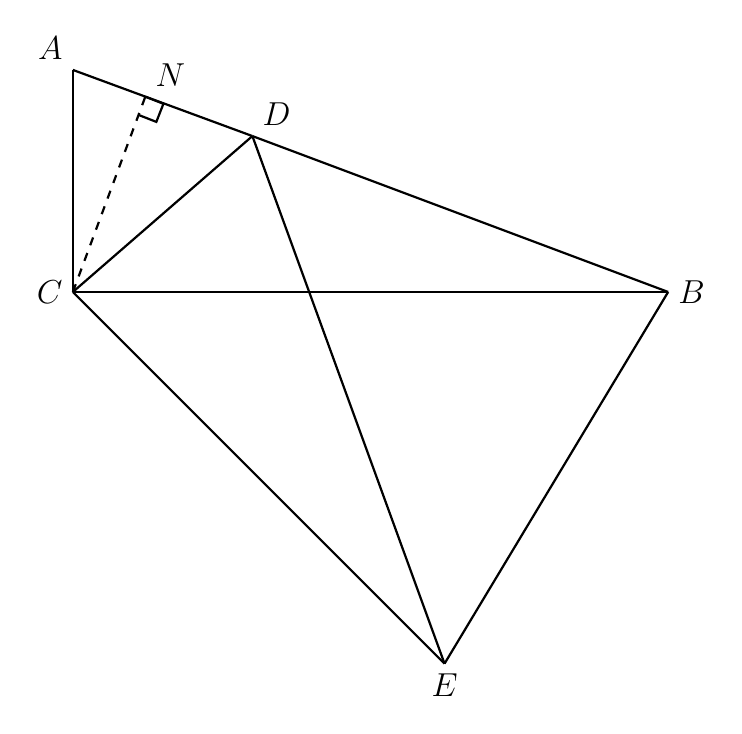
\begin{tikzpicture}[line width=0.8pt, font=\large]
  \coordinate (A) at (0,2.82);
  \coordinate (C) at (0,0);
  \coordinate (B) at (7.56,0);
  \coordinate (D) at (2.28,1.98);
  \coordinate (E) at (4.72,-4.72);
  \coordinate (N) at (0.92,2.48);

  \draw (A) -- (C);
  \draw (A) -- (D);
  \draw (D) -- (B);
  \draw (C) -- (B);
  \draw (C) -- (D);
  \draw (C) -- (E);
  \draw (D) -- (E);
  \draw (E) -- (B);
  \draw[dashed] (C) -- (N);

  \draw (N) -- (1.15,2.39) -- (1.06,2.16) -- (0.83,2.25);

  \node[above left] at (A) {$A$};
  \node[above right] at (N) {$N$};
  \node[above right] at (D) {$D$};
  \node[right] at (B) {$B$};
  \node[left] at (C) {$C$};
  \node[below] at (E) {$E$};
\end{tikzpicture}
\end{document}
